% =============================================================================
% Pipeline flowcharts for
%   "Automated Detection of Ignored Clustering and Restricted Randomization
%    in Trials with Clusters"
%
% Compile:  pdflatex pipeline_flowchart.tex
% One page per figure (standalone), each sized to its content. Drop each page
% straight into a slide.
%
%   Page 1  Overview: the six-stage workflow
%   Page 2  Stage 2, Data collection and preparation
%   Page 3  Stage 3, Promptbook development (the loop)
%   Page 4  Stage 3 detail, how a miss becomes a rule
%   Page 5  Stages 4 and 5, Processing and validation
%   Page 6  Legend
%
% Stage numbers follow Zupic (2026), A Human-Centered Workflow for Using Large
% Language Models in Content Analysis:
%   1 Research design                    4 Processing
%   2 Data collection and preparation    5 Assessing validity/reliability
%   3 Promptbook development             6 Interpretation and further analysis
%
% Export PNGs:  pdftoppm -r 300 -png pipeline_flowchart.pdf stage
% =============================================================================
\documentclass[tikz,border=14pt]{standalone}

\usepackage[T1]{fontenc}
\usepackage{lmodern}
\usetikzlibrary{positioning, arrows.meta, fit, backgrounds, calc}

% ----- palette ---------------------------------------------------------------
\definecolor{ink}{HTML}{151C22}      % text
\definecolor{model}{HTML}{1F5E66}    % steps the MODEL performs
\definecolor{human}{HTML}{8A4F7D}    % steps a HUMAN performs
\definecolor{store}{HTML}{54636D}    % data stores
\definecolor{done}{HTML}{2E6B4F}     % completed / final outputs
\definecolor{drop}{HTML}{A03E28}     % papers leaving
\definecolor{band}{HTML}{EEF2F3}     % panel background

% ----- styles (pf* prefix: plain names like `cap` collide with TikZ keys) -----
\tikzset{
  every node/.style = {font=\sffamily, text=ink},
  pfbase/.style   = {draw, line width=0.9pt, fill=white, align=center, inner sep=5pt,
                     rounded corners=1.5pt, font=\sffamily\small, minimum height=10mm},
  pfmodel/.style  = {pfbase, draw=model},
  pfhuman/.style  = {pfbase, draw=human, fill=human!6},
  pfstore/.style  = {pfbase, draw=store, densely dashed, fill=store!5},
  pfdone/.style   = {pfbase, draw=done, fill=done!8, line width=1.3pt},
  pfdrop/.style   = {pfbase, draw=drop, densely dotted, fill=drop!5, font=\sffamily\scriptsize},
  pfnum/.style    = {pfbase, draw=model, fill=model!8, line width=1.3pt, font=\sffamily\small\bfseries},
  pfgo/.style     = {-{Latex[length=2.4mm,width=1.8mm]}, draw=model, line width=1pt},
  pfgoh/.style    = {-{Latex[length=2.4mm,width=1.8mm]}, draw=human, line width=1pt},
  pfout/.style    = {-{Latex[length=2mm,width=1.5mm]}, draw=drop, line width=0.7pt, densely dotted},
  pffeed/.style   = {-{Latex[length=2.4mm,width=1.8mm]}, draw=store, line width=0.9pt, densely dashed},
  pfcap/.style    = {font=\sffamily\scriptsize, text=store, align=center},
  pflab/.style    = {font=\sffamily\scriptsize, text=store, fill=white, inner sep=1.5pt},
  pfstep/.style   = {circle, draw=model, line width=1pt, fill=white, inner sep=0pt,
                     minimum size=7mm, font=\sffamily\bfseries\small, text=model},
  pfhead/.style   = {font=\sffamily\bfseries\Large, text=ink, anchor=west, align=left},
  pfsub/.style    = {font=\sffamily\small, text=store, anchor=west, align=left},
  pfeyebrow/.style= {font=\sffamily\bfseries\small, text=model, anchor=west},
}

% shorthand: an "in:" tag marking input carried from another stage
\newcommand{\pfin}[1]{{\itshape in: #1}}

\begin{document}

% =============================================================================
% PAGE 1  OVERVIEW
% =============================================================================
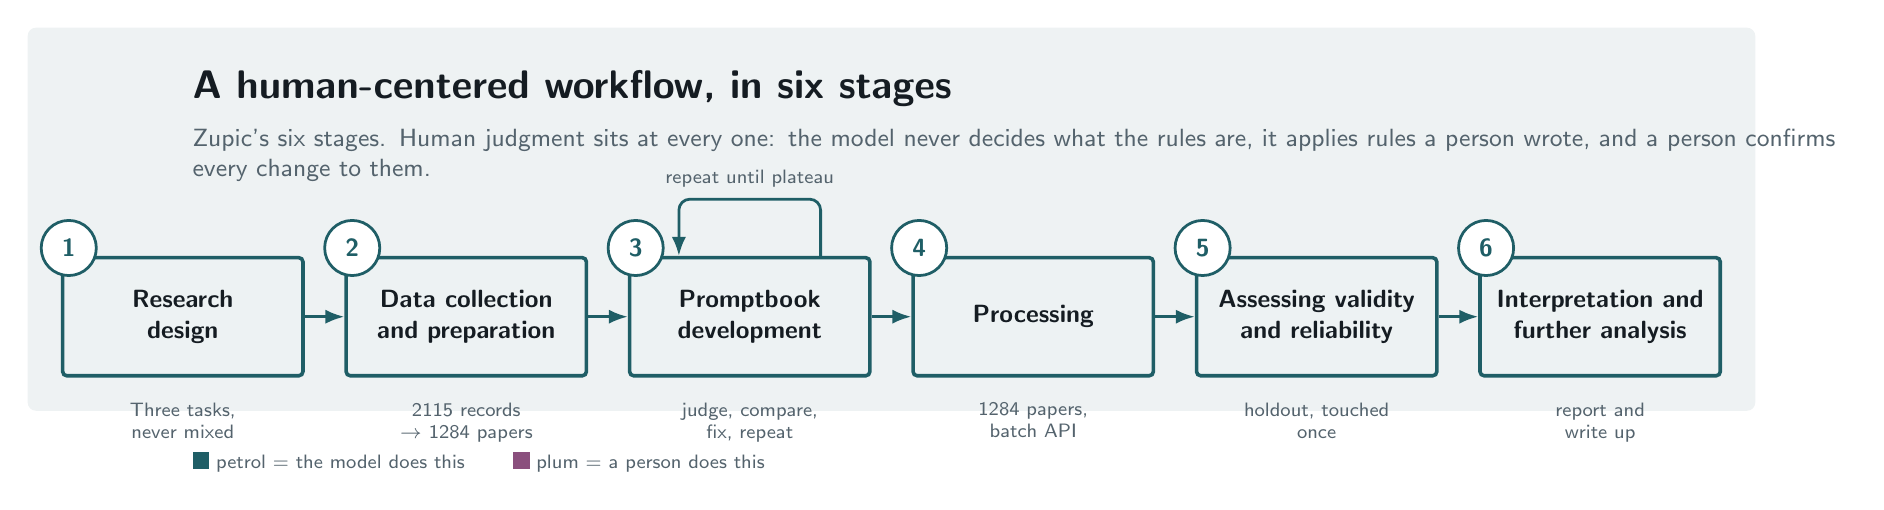
\begin{tikzpicture}

\node[pfhead] (T) at (0,2.0) {A human-centered workflow, in six stages};
\node[pfsub, text width=21cm] at (0,1.15)
  {Zupic's six stages. Human judgment sits at every one: the model never decides what the rules
   are, it applies rules a person wrote, and a person confirms every change to them.};

\foreach \i/\x/\ttl/\sub in {%
  1/0/{Research\\design}/{Three tasks,\\never mixed},
  2/3.6/{Data collection\\and preparation}/{2115 records\\$\rightarrow$ 1284 papers},
  3/7.2/{Promptbook\\development}/{judge, compare,\\fix, repeat},
  4/10.8/{Processing}/{1284 papers,\\batch API},
  5/14.4/{Assessing validity\\and reliability}/{holdout, touched\\once},
  6/18.0/{Interpretation and\\further analysis}/{report and\\write up}%
}{
  \node[pfnum, text width=2.7cm, minimum height=15mm] (S\i) at (\x,-0.9) {\ttl};
  \node[pfstep] at ($(S\i.north west)+(0.1,0.1)$) {\i};
  \node[pfcap, below=2mm of S\i, text width=2.9cm] {\sub};
}
\foreach \a/\b in {1/2,2/3,3/4,4/5,5/6}{\draw[pfgo] (S\a) -- (S\b);}

\draw[pfgo, rounded corners=4pt]
  ($(S3.north)+(0.9,0)$) -- ++(0,0.72) -- ++(-1.8,0) -- ($(S3.north)+(-0.9,0)$);
\node[pfcap, above=7.5mm of S3] {repeat until plateau};

\node[pfcap, anchor=west, align=left] at (0,-2.75)
  {\textcolor{model}{\rule{6pt}{6pt}}~petrol = the model does this
   \qquad \textcolor{human}{\rule{6pt}{6pt}}~plum = a person does this};

\begin{scope}[on background layer]
  \node[fill=band, rounded corners=3pt, fit=(T)(S1)(S6), inner sep=12pt] {};
\end{scope}
\end{tikzpicture}


% =============================================================================
% PAGE 2  STAGE 2  DATA COLLECTION AND PREPARATION
% =============================================================================
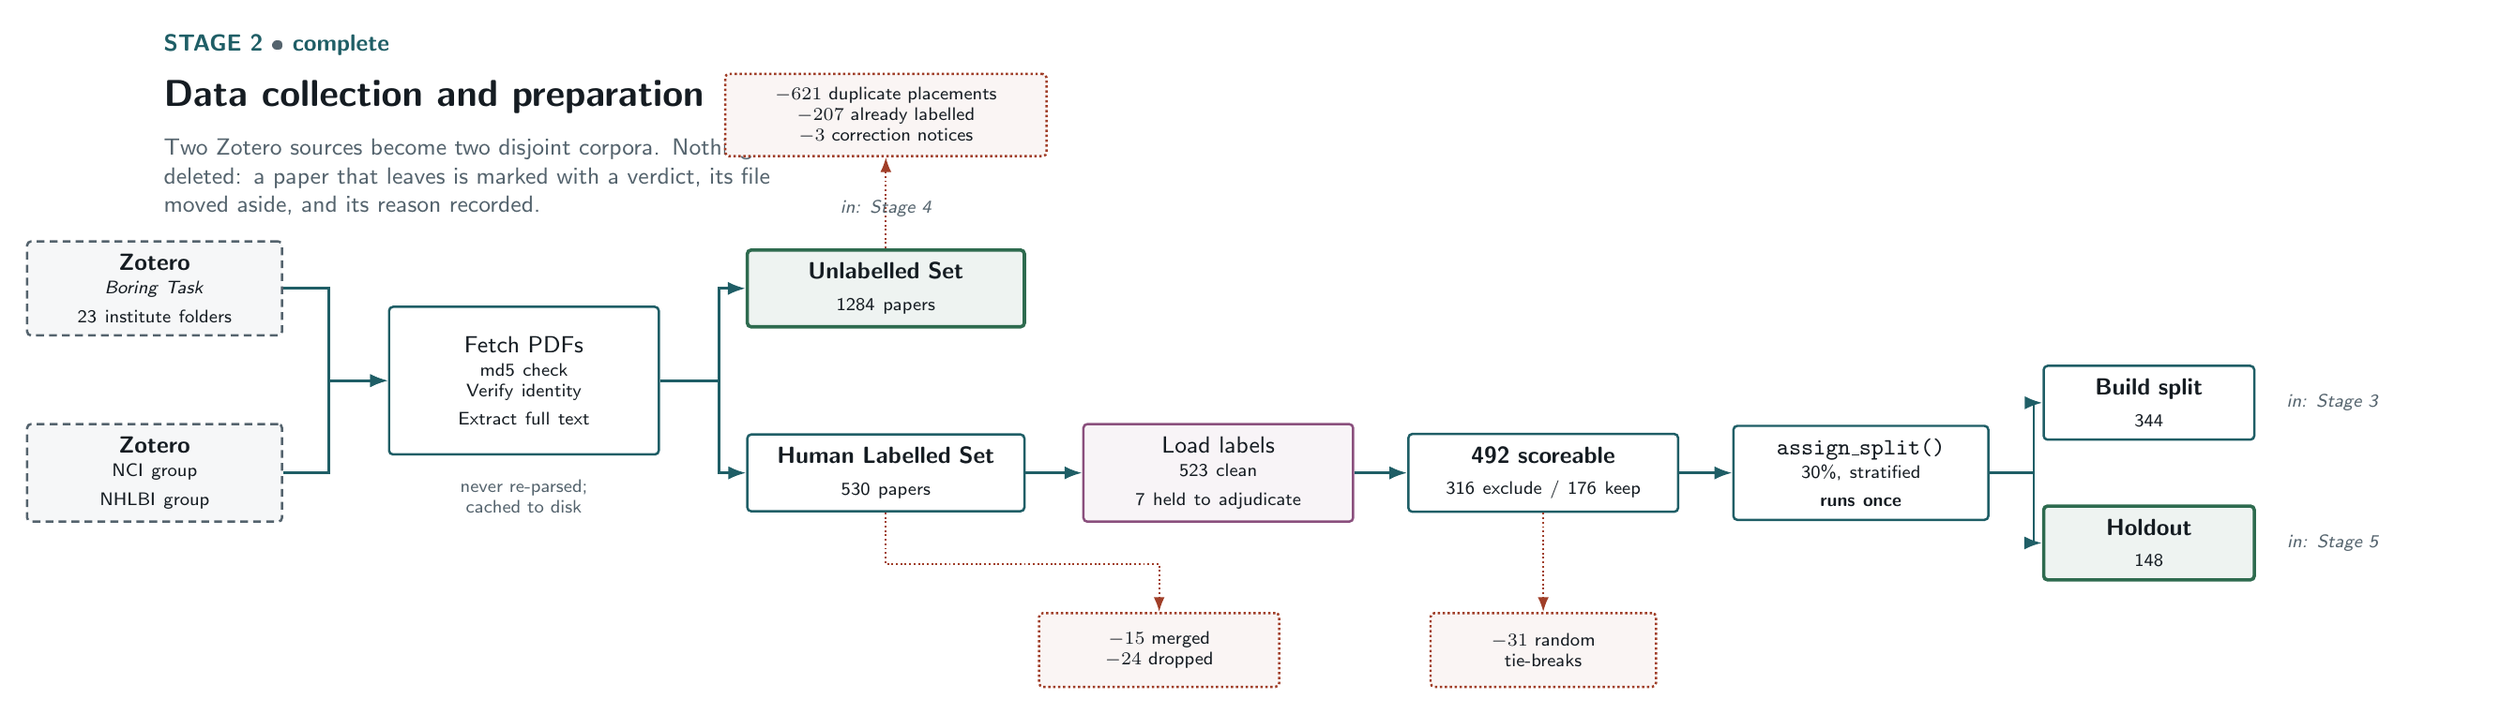
\begin{tikzpicture}

\node[pfeyebrow] at (0,3.3) {STAGE 2 \textcolor{store}{\textbullet} complete};
\node[pfhead]    at (0,2.6) {Data collection and preparation};
\node[pfsub, text width=8.6cm, anchor=north west] at (0,2.15)
  {Two Zotero sources become two disjoint corpora. Nothing is deleted: a paper that leaves is
   marked with a verdict, its file moved aside, and its reason recorded.};

\node[pfstore, text width=3.1cm] (zA) at (0,0)
  {\textbf{Zotero}\\[1pt]\scriptsize \emph{Boring Task}\\23 institute folders};
\node[pfstore, text width=3.1cm] (zB) at (0,-2.5)
  {\textbf{Zotero}\\[1pt]\scriptsize NCI group\\NHLBI group};

\node[pfmodel, text width=3.3cm, minimum height=20mm] (prep) at (5.0,-1.25)
  {Fetch PDFs\\[1pt]\scriptsize md5 check\\Verify identity\\Extract full text};
\node[pfcap, below=2mm of prep, text width=3.6cm] {never re-parsed;\\cached to disk};

\node[pfdone,  text width=3.4cm] (unl) at (9.9,0)
  {\textbf{Unlabelled Set}\\[1pt]\scriptsize 1284 papers};
\node[pfmodel, text width=3.4cm] (lab) at (9.9,-2.5)
  {\textbf{Human Labelled Set}\\[1pt]\scriptsize 530 papers};

\node[pfhuman, text width=3.3cm] (load) at (14.4,-2.5)
  {Load labels\\[1pt]\scriptsize 523 clean\\7 held to adjudicate};
\node[pfmodel, text width=3.3cm] (scor) at (18.8,-2.5)
  {\textbf{492 scoreable}\\[1pt]\scriptsize 316 exclude / 176 keep};
\node[pfmodel, text width=3.1cm] (splt) at (23.1,-2.5)
  {\texttt{assign\_split()}\\[1pt]\scriptsize 30\%, stratified\\\textbf{runs once}};

\node[pfmodel, text width=2.5cm] (bld) at (27.0,-1.55) {\textbf{Build split}\\[1pt]\scriptsize 344};
\node[pfdone,  text width=2.5cm] (hld) at (27.0,-3.45) {\textbf{Holdout}\\[1pt]\scriptsize 148};

\node[pfdrop, text width=4.0cm] (d1) at (9.9,2.35)
  {$-621$ duplicate placements\\$-207$ already labelled\\$-3$ correction notices};
\node[pfdrop, text width=2.9cm] (d2) at (13.6,-4.9) {$-15$ merged\\$-24$ dropped};
\node[pfdrop, text width=2.7cm] (d3) at (18.8,-4.9) {$-31$ random\\tie-breaks};

\draw[pfgo] (zA) -| ($(prep.west)+(-8mm,0)$) |- (prep.west);
\draw[pfgo] (zB) -| ($(prep.west)+(-8mm,0)$) |- (prep.west);
\draw[pfgo] (prep.east) -- ($(prep.east)+(8mm,0)$) |- (unl.west);
\draw[pfgo] (prep.east) -- ($(prep.east)+(8mm,0)$) |- (lab.west);
\draw[pfgo] (lab)  -- (load);
\draw[pfgo] (load) -- (scor);
\draw[pfgo] (scor) -- (splt);
\draw[pfgo] (splt.east) -- ($(splt.east)+(6mm,0)$) |- (bld.west);
\draw[pfgo] (splt.east) -- ($(splt.east)+(6mm,0)$) |- (hld.west);
\draw[pfout] (unl)  -- (d1);
\draw[pfout] (lab.south) -- ++(0,-7mm) -| (d2.north);
\draw[pfout] (scor) -- (d3);

\node[pfcap, right=3mm of bld, text width=2.4cm, align=left] {\pfin{Stage 3}};
\node[pfcap, right=3mm of hld, text width=2.4cm, align=left] {\pfin{Stage 5}};
\node[pfcap, above=3mm of unl, text width=3.6cm] {\pfin{Stage 4}};
\end{tikzpicture}


% =============================================================================
% PAGE 3  STAGE 3  PROMPTBOOK DEVELOPMENT
% =============================================================================
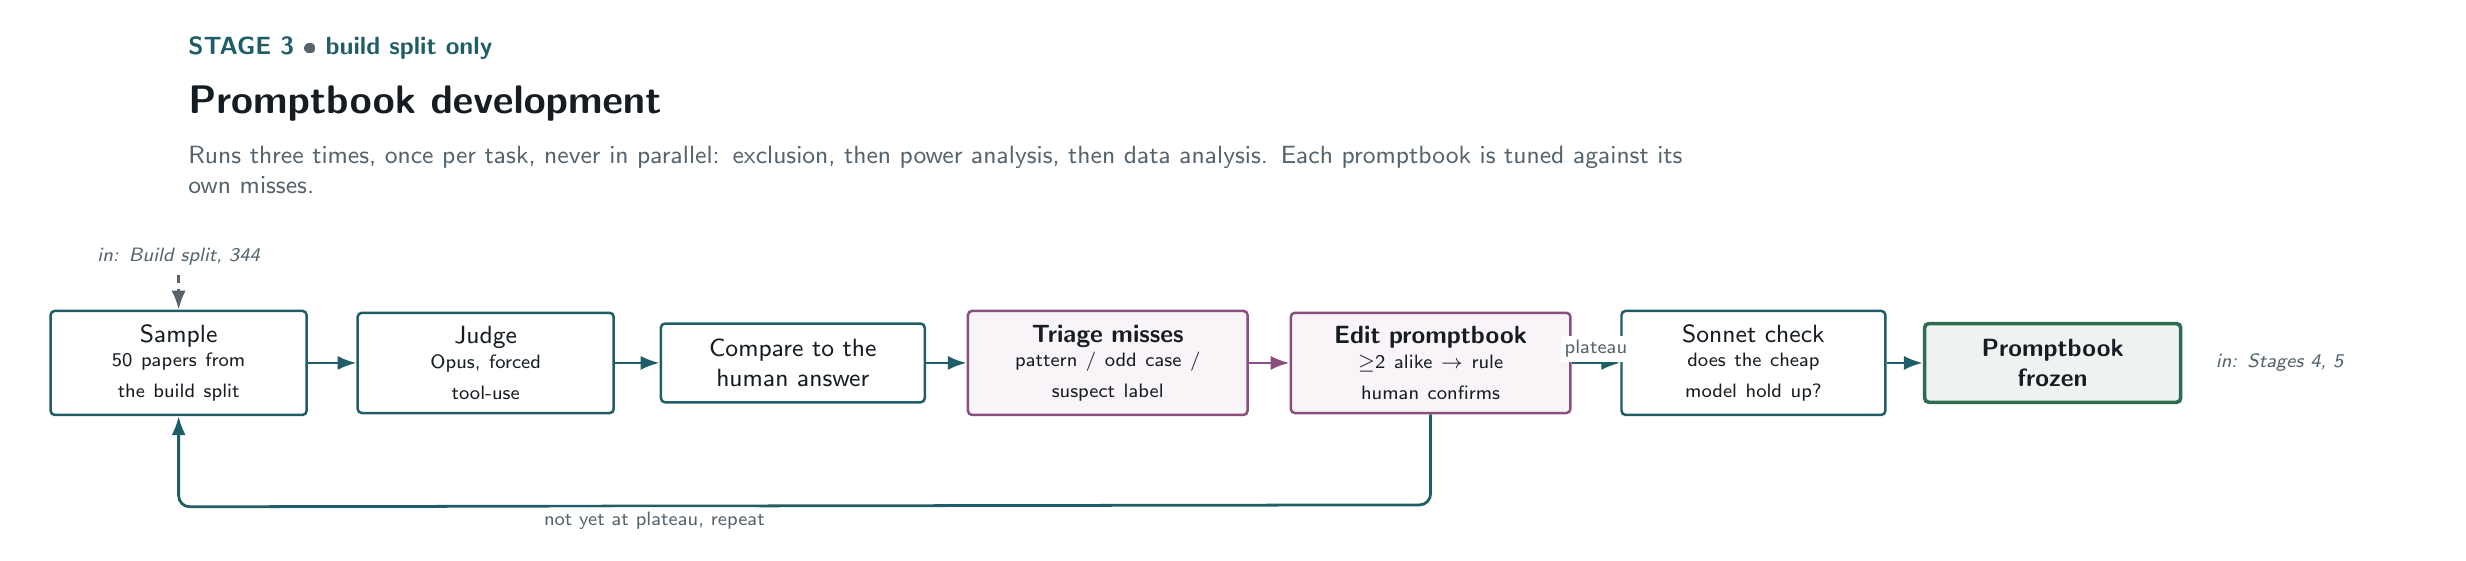
\begin{tikzpicture}

\node[pfeyebrow] at (0,3.0) {STAGE 3 \textcolor{store}{\textbullet} build split only};
\node[pfhead]    at (0,2.3) {Promptbook development};
\node[pfsub, text width=19cm] at (0,1.45)
  {Runs three times, once per task, never in parallel: exclusion, then power analysis, then data
   analysis. Each promptbook is tuned against its own misses.};

\node[pfcap, text width=3.6cm] (feedin) at (0,0.35) {\pfin{Build split, 344}};

\node[pfmodel, text width=2.9cm] (samp) at (0,-1.0)
  {Sample\\[1pt]\scriptsize 50 papers from\\the build split};
\node[pfmodel, text width=2.9cm] (judg) at (3.9,-1.0)
  {Judge\\[1pt]\scriptsize Opus, forced\\tool-use};
\node[pfmodel, text width=3.0cm] (comp) at (7.8,-1.0)
  {Compare to the\\human answer};
\node[pfhuman, text width=3.2cm] (tri)  at (11.8,-1.0)
  {\textbf{Triage misses}\\[1pt]\scriptsize pattern / odd case /\\suspect label};
\node[pfhuman, text width=3.2cm] (edt)  at (15.9,-1.0)
  {\textbf{Edit promptbook}\\[1pt]\scriptsize $\geq$2 alike $\rightarrow$ rule\\human confirms};
\node[pfmodel, text width=3.0cm] (son)  at (20.0,-1.0)
  {Sonnet check\\[1pt]\scriptsize does the cheap\\model hold up?};
\node[pfdone,  text width=2.9cm] (frz)  at (23.8,-1.0)
  {\textbf{Promptbook}\\\textbf{frozen}};

\draw[pffeed] (feedin) -- (samp);
\foreach \a/\b in {samp/judg, judg/comp, comp/tri}{\draw[pfgo] (\a) -- (\b);}
\draw[pfgoh] (tri) -- (edt);
\draw[pfgo]  (edt) -- node[pflab, above]{plateau} (son);
\draw[pfgo]  (son) -- (frz);

\draw[pfgo, rounded corners=4pt]
  (edt.south) -- ++(0,-1.15)
  -- node[pflab, below, pos=0.62]{not yet at plateau, repeat}
     ($(samp.south)+(0,-1.15)$) -- (samp.south);

\node[pfcap, right=3mm of frz, text width=2.7cm, align=left] {\pfin{Stages 4, 5}};
\end{tikzpicture}


% =============================================================================
% PAGE 4  STAGE 3 DETAIL  HOW A MISS BECOMES A RULE
% =============================================================================
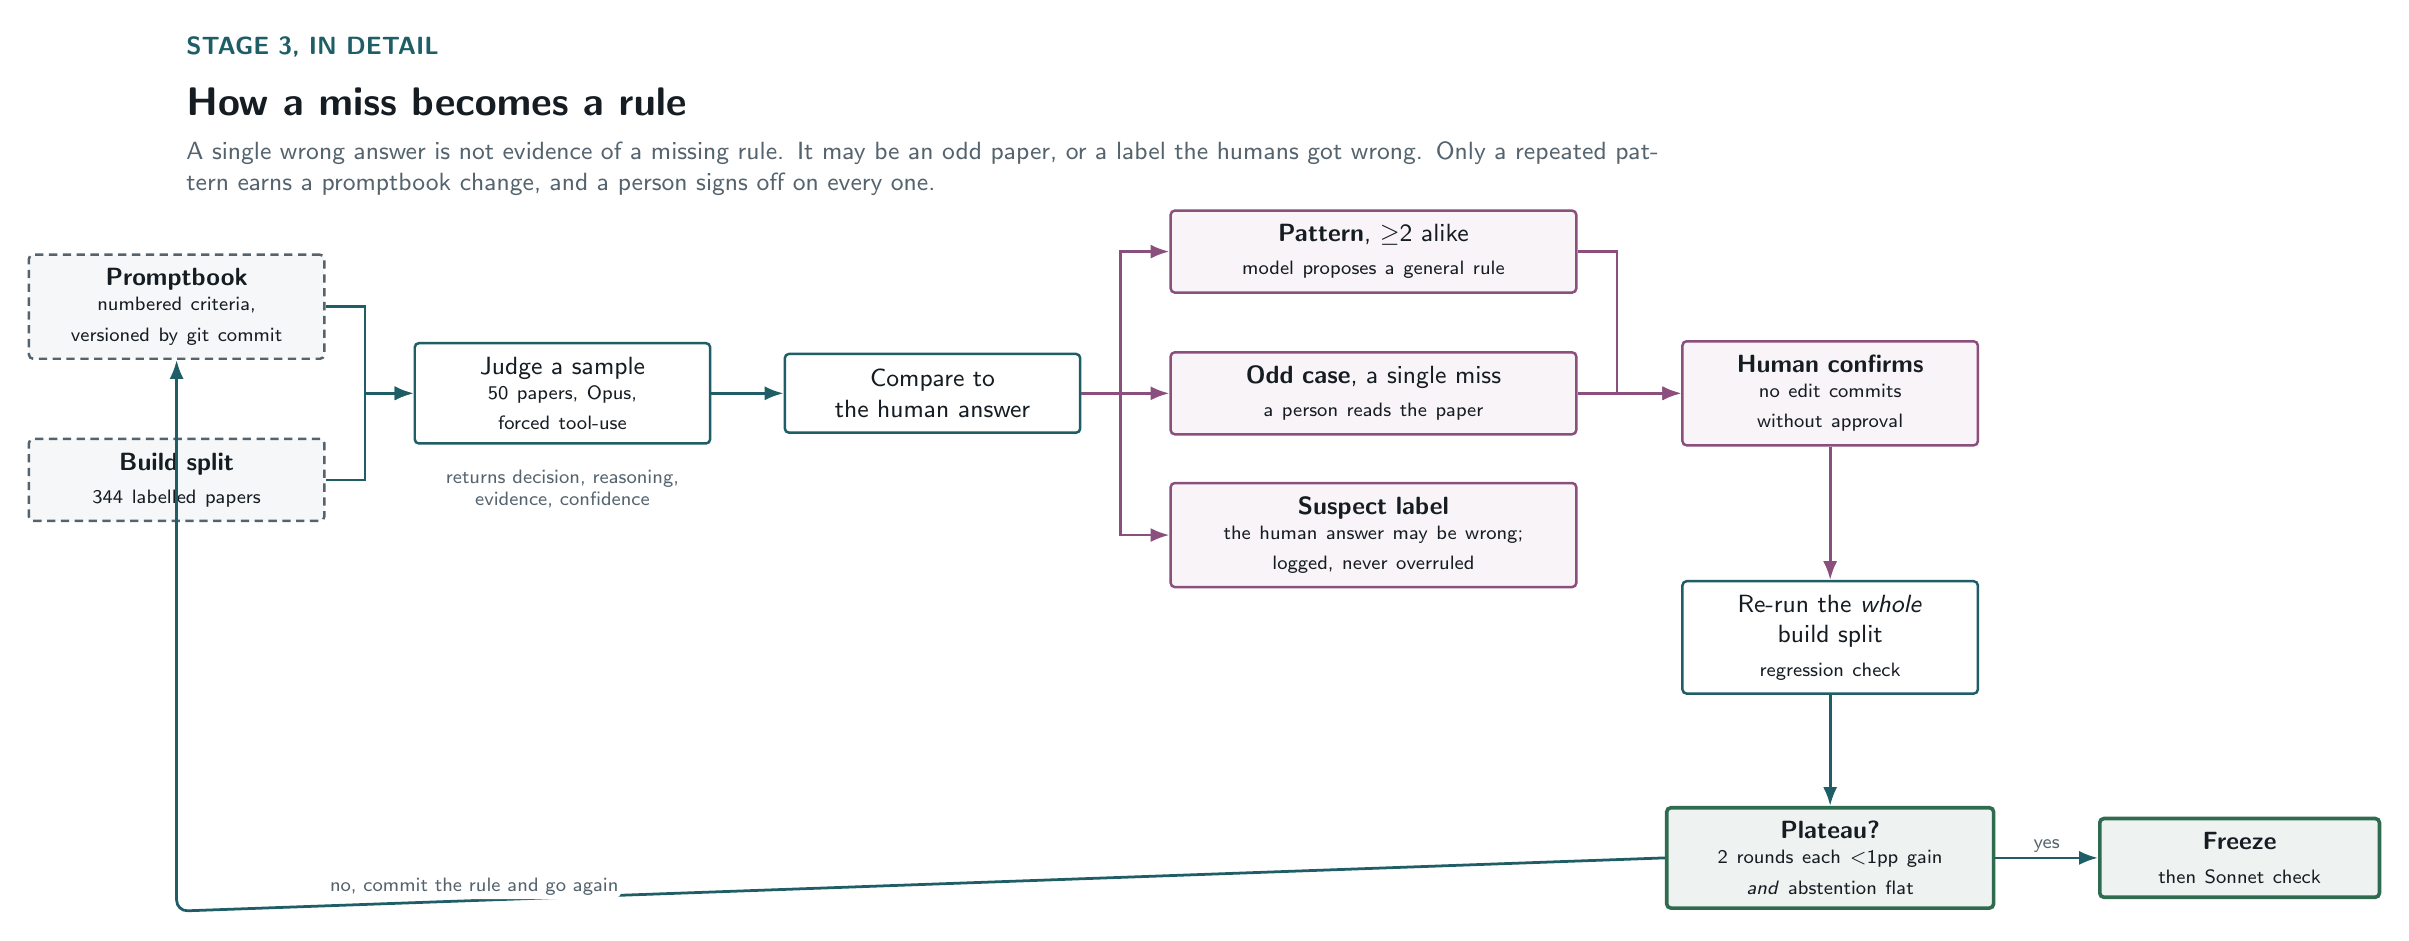
\begin{tikzpicture}

\node[pfeyebrow] at (0,3.3) {STAGE 3, IN DETAIL};
\node[pfhead]    at (0,2.6) {How a miss becomes a rule};
\node[pfsub, text width=19cm] at (0,1.75)
  {A single wrong answer is not evidence of a missing rule. It may be an odd paper, or a label the
   humans got wrong. Only a repeated pattern earns a promptbook change, and a person signs off on
   every one.};

\node[pfstore, text width=3.4cm] (pb) at (0,0)
  {\textbf{Promptbook}\\[1pt]\scriptsize numbered criteria,\\versioned by git commit};
\node[pfstore, text width=3.4cm] (bs) at (0,-2.2)
  {\textbf{Build split}\\[1pt]\scriptsize 344 labelled papers};

\node[pfmodel, text width=3.4cm] (run) at (4.9,-1.1)
  {Judge a sample\\[1pt]\scriptsize 50 papers, Opus,\\forced tool-use};
\node[pfcap, below=2mm of run, text width=4.2cm]
  {returns decision, reasoning,\\evidence, confidence};

\node[pfmodel, text width=3.4cm] (cmp) at (9.6,-1.1) {Compare to\\the human answer};

\node[pfhuman, text width=4.8cm] (t1) at (15.2,0.7)
  {\textbf{Pattern}, $\geq$2 alike\\[1pt]\scriptsize model proposes a general rule};
\node[pfhuman, text width=4.8cm] (t2) at (15.2,-1.1)
  {\textbf{Odd case}, a single miss\\[1pt]\scriptsize a person reads the paper};
\node[pfhuman, text width=4.8cm] (t3) at (15.2,-2.9)
  {\textbf{Suspect label}\\[1pt]\scriptsize the human answer may be wrong;\\logged, never overruled};

\node[pfhuman, text width=3.4cm] (cfm) at (21.0,-1.1)
  {\textbf{Human confirms}\\[1pt]\scriptsize no edit commits\\without approval};
\node[pfmodel, text width=3.4cm] (reg) at (21.0,-4.2)
  {Re-run the \emph{whole}\\build split\\[1pt]\scriptsize regression check};
\node[pfdone, text width=3.8cm] (plt) at (21.0,-7.0)
  {\textbf{Plateau?}\\[1pt]\scriptsize 2 rounds each $<$1pp gain\\\emph{and} abstention flat};
\node[pfdone, text width=3.2cm] (out) at (26.2,-7.0)
  {\textbf{Freeze}\\[1pt]\scriptsize then Sonnet check};

\draw[pfgo] (pb.east) -- ++(5mm,0) |- (run.west);
\draw[pfgo] (bs.east) -- ++(5mm,0) |- (run.west);
\draw[pfgo] (run) -- (cmp);
\foreach \t in {t1,t2,t3}{\draw[pfgoh] (cmp.east) -- ++(5mm,0) |- (\t.west);}
\draw[pfgoh] (t1.east) -- ++(5mm,0) |- (cfm.west);
\draw[pfgoh] (t2.east) -- ++(5mm,0) |- (cfm.west);
\draw[pfgoh] (cfm) -- (reg);
\draw[pfgo]  (reg) -- (plt);
\draw[pfgo]  (plt) -- node[pflab, above]{yes} (out);
\draw[pfgo, rounded corners=4pt]
  (plt.west) -- node[pflab, above, pos=0.80]{no, commit the rule and go again}
  ($(pb.south)+(0,-7.0)$) -- (pb.south);
\end{tikzpicture}


% =============================================================================
% PAGE 5  STAGES 4 AND 5  PROCESSING AND VALIDATION
% =============================================================================
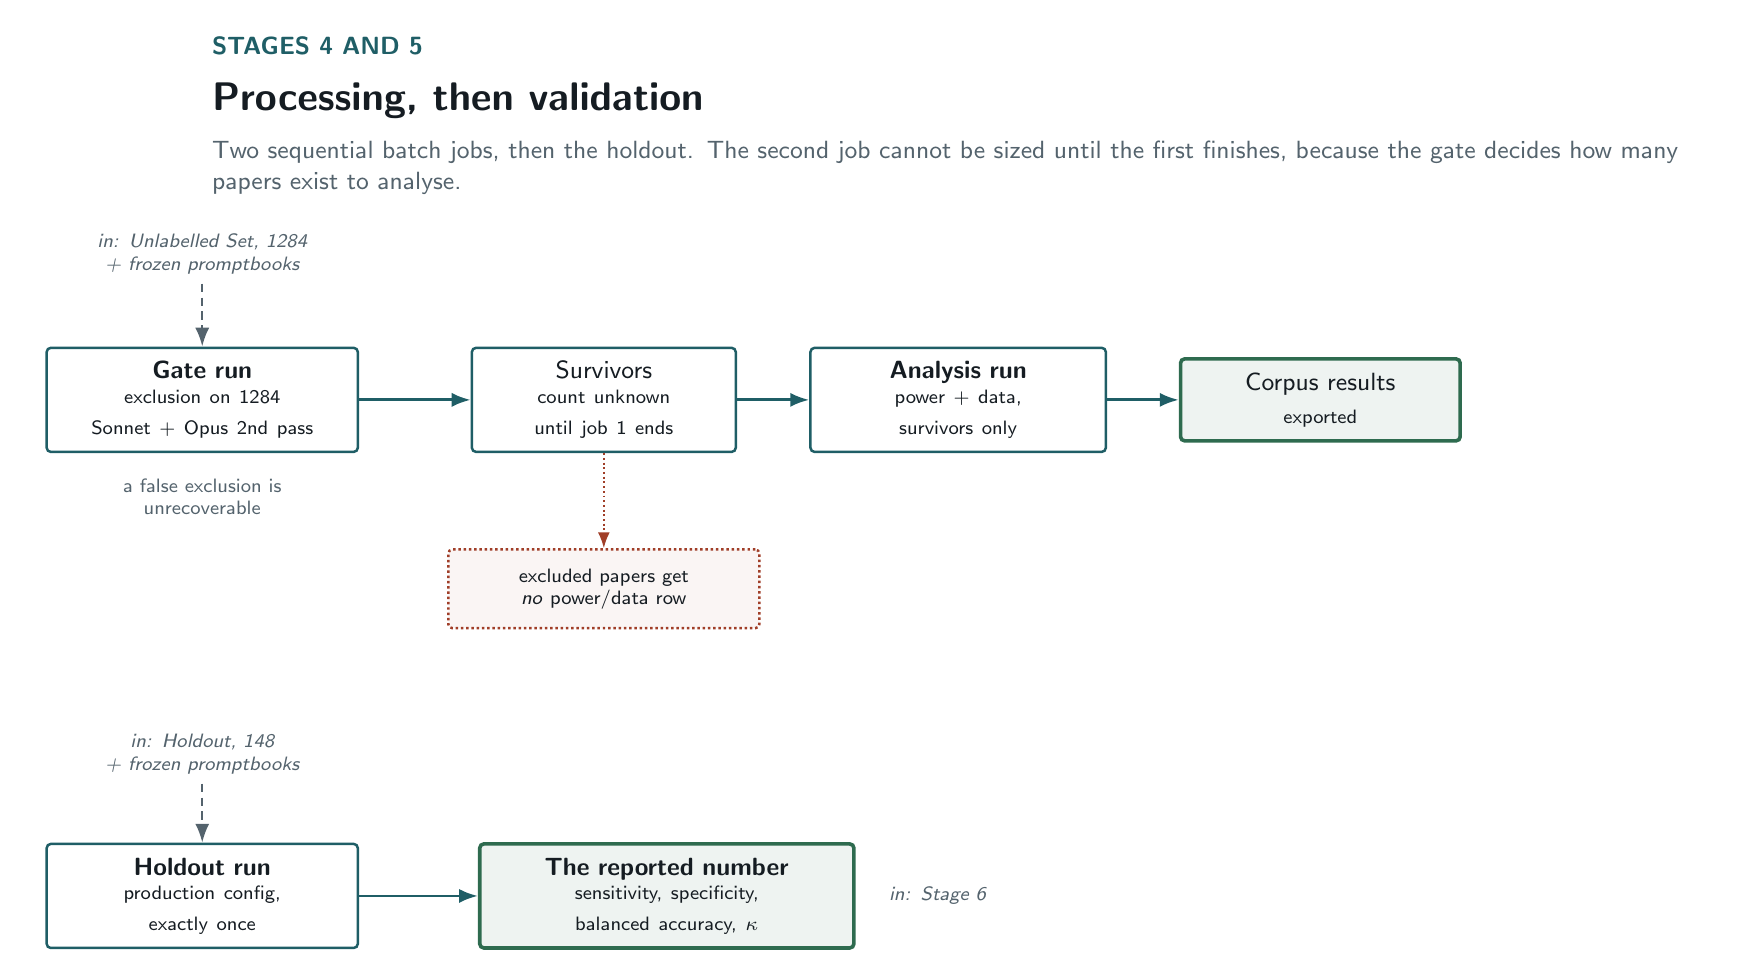
\begin{tikzpicture}

\node[pfeyebrow] at (0,3.0) {STAGES 4 AND 5};
\node[pfhead]    at (0,2.3) {Processing, then validation};
\node[pfsub, text width=19cm] at (0,1.45)
  {Two sequential batch jobs, then the holdout. The second job cannot be sized until the first
   finishes, because the gate decides how many papers exist to analyse.};

\node[pfcap, text width=4.2cm] (in1) at (0,0.35)
  {\pfin{Unlabelled Set, 1284\\+ frozen promptbooks}};

\node[pfmodel, text width=3.6cm] (gate) at (0,-1.5)
  {\textbf{Gate run}\\[1pt]\scriptsize exclusion on 1284\\Sonnet + Opus 2nd pass};
\node[pfmodel, text width=3.0cm] (surv) at (5.1,-1.5)
  {Survivors\\[1pt]\scriptsize count unknown\\until job 1 ends};
\node[pfmodel, text width=3.4cm] (anal) at (9.6,-1.5)
  {\textbf{Analysis run}\\[1pt]\scriptsize power + data,\\survivors only};
\node[pfdone, text width=3.2cm] (res) at (14.2,-1.5)
  {Corpus results\\[1pt]\scriptsize exported};

\node[pfcap, below=2mm of gate, text width=4.2cm]
  {a false exclusion is\\unrecoverable};
\node[pfdrop, text width=3.6cm] (gd) at (5.1,-3.9)
  {excluded papers get\\\emph{no} power/data row};

\node[pfcap, text width=4.2cm] (in2) at (0,-6.0)
  {\pfin{Holdout, 148\\+ frozen promptbooks}};
\node[pfmodel, text width=3.6cm] (hrun) at (0,-7.8)
  {\textbf{Holdout run}\\[1pt]\scriptsize production config,\\exactly once};
\node[pfdone, text width=4.4cm] (fin) at (5.9,-7.8)
  {\textbf{The reported number}\\[1pt]\scriptsize sensitivity, specificity,\\balanced accuracy, $\kappa$};

\draw[pffeed] (in1) -- (gate);
\draw[pfgo] (gate) -- (surv);
\draw[pfgo] (surv) -- (anal);
\draw[pfgo] (anal) -- (res);
\draw[pfout] (surv) -- (gd);
\draw[pffeed] (in2) -- (hrun);
\draw[pfgo] (hrun) -- (fin);

\node[pfcap, right=3mm of fin, text width=3.0cm, align=left] {\pfin{Stage 6}};
\end{tikzpicture}


% =============================================================================
% PAGE 6  LEGEND
% =============================================================================
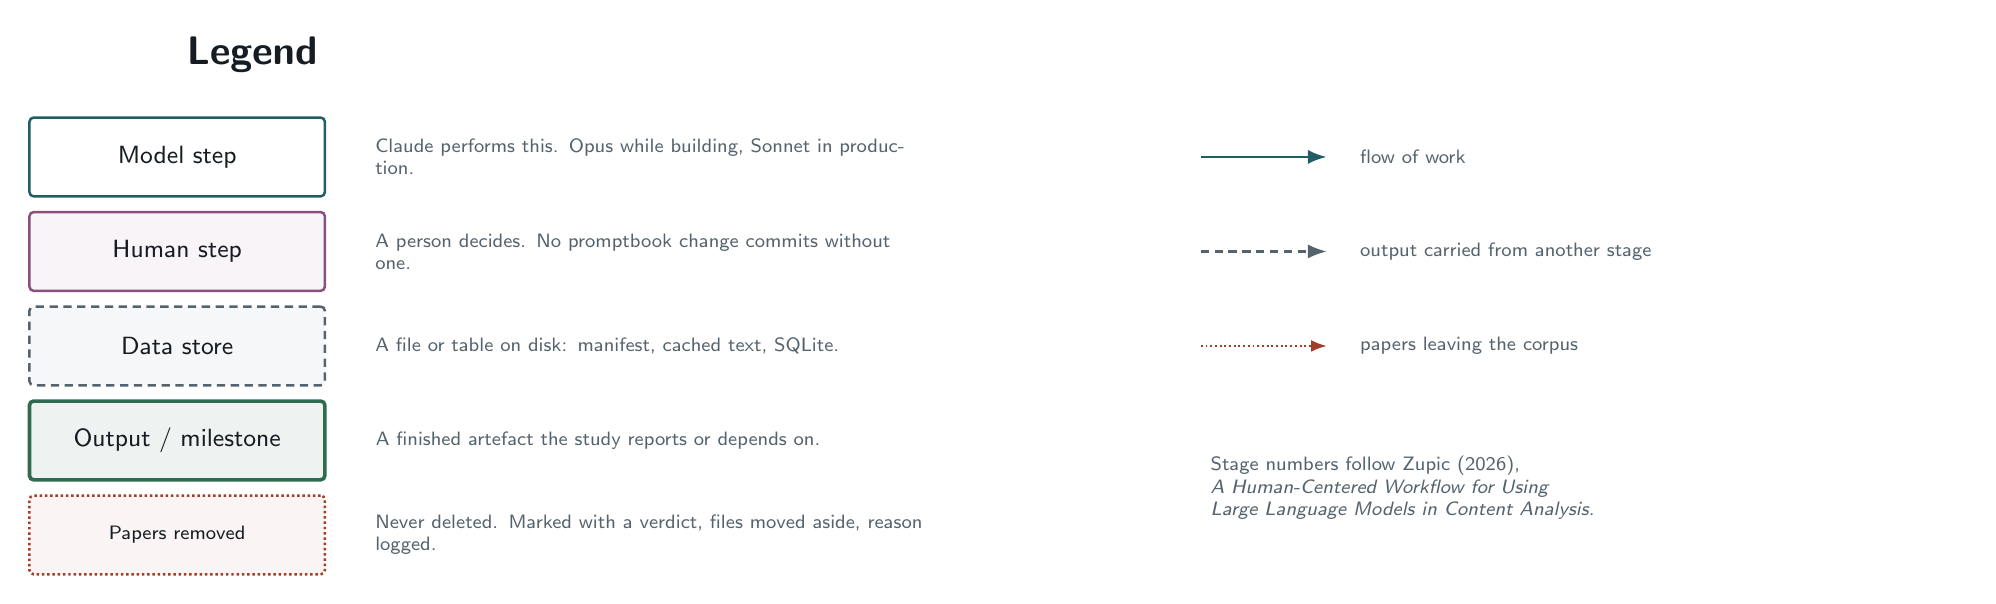
\begin{tikzpicture}

\node[pfhead] at (0,2.6) {Legend};

\node[pfmodel, text width=3.4cm] (l1) at (0,1.3) {Model step};
\node[pfcap, right=5mm of l1, text width=7.0cm, align=left]
  {Claude performs this. Opus while building, Sonnet in production.};

\node[pfhuman, text width=3.4cm] (l2) at (0,0.1) {Human step};
\node[pfcap, right=5mm of l2, text width=7.0cm, align=left]
  {A person decides. No promptbook change commits without one.};

\node[pfstore, text width=3.4cm] (l3) at (0,-1.1) {Data store};
\node[pfcap, right=5mm of l3, text width=7.0cm, align=left]
  {A file or table on disk: manifest, cached text, SQLite.};

\node[pfdone, text width=3.4cm] (l4) at (0,-2.3) {Output / milestone};
\node[pfcap, right=5mm of l4, text width=7.0cm, align=left]
  {A finished artefact the study reports or depends on.};

\node[pfdrop, text width=3.4cm] (l5) at (0,-3.5) {Papers removed};
\node[pfcap, right=5mm of l5, text width=7.0cm, align=left]
  {Never deleted. Marked with a verdict, files moved aside, reason logged.};

\draw[pfgo]   (13.0,1.3)  -- (14.6,1.3);
\node[pfcap, anchor=west, text width=6.4cm, align=left] at (14.9,1.3)  {flow of work};
\draw[pffeed] (13.0,0.1)  -- (14.6,0.1);
\node[pfcap, anchor=west, text width=6.4cm, align=left] at (14.9,0.1)  {output carried from another stage};
\draw[pfout]  (13.0,-1.1) -- (14.6,-1.1);
\node[pfcap, anchor=west, text width=6.4cm, align=left] at (14.9,-1.1) {papers leaving the corpus};

\node[pfcap, anchor=west, text width=9.5cm, align=left] at (13.0,-2.9)
  {Stage numbers follow Zupic (2026),\\\emph{A Human-Centered Workflow for Using\\Large Language
   Models in Content Analysis}.};
\end{tikzpicture}

\end{document}
